
\documentclass[11pt]{article}\usepackage[]{graphicx}\usepackage[]{color}
%% maxwidth is the original width if it is less than linewidth
%% otherwise use linewidth (to make sure the graphics do not exceed the margin)
\makeatletter
\def\maxwidth{ %
  \ifdim\Gin@nat@width>\linewidth
    \linewidth
  \else
    \Gin@nat@width
  \fi
}
\makeatother

\definecolor{fgcolor}{rgb}{0.345, 0.345, 0.345}
\newcommand{\hlnum}[1]{\textcolor[rgb]{0.686,0.059,0.569}{#1}}%
\newcommand{\hlstr}[1]{\textcolor[rgb]{0.192,0.494,0.8}{#1}}%
\newcommand{\hlcom}[1]{\textcolor[rgb]{0.678,0.584,0.686}{\textit{#1}}}%
\newcommand{\hlopt}[1]{\textcolor[rgb]{0,0,0}{#1}}%
\newcommand{\hlstd}[1]{\textcolor[rgb]{0.345,0.345,0.345}{#1}}%
\newcommand{\hlkwa}[1]{\textcolor[rgb]{0.161,0.373,0.58}{\textbf{#1}}}%
\newcommand{\hlkwb}[1]{\textcolor[rgb]{0.69,0.353,0.396}{#1}}%
\newcommand{\hlkwc}[1]{\textcolor[rgb]{0.333,0.667,0.333}{#1}}%
\newcommand{\hlkwd}[1]{\textcolor[rgb]{0.737,0.353,0.396}{\textbf{#1}}}%

\usepackage{framed}
\makeatletter
\newenvironment{kframe}{%
 \def\at@end@of@kframe{}%
 \ifinner\ifhmode%
  \def\at@end@of@kframe{\end{minipage}}%
  \begin{minipage}{\columnwidth}%
 \fi\fi%
 \def\FrameCommand##1{\hskip\@totalleftmargin \hskip-\fboxsep
 \colorbox{shadecolor}{##1}\hskip-\fboxsep
     % There is no \\@totalrightmargin, so:
     \hskip-\linewidth \hskip-\@totalleftmargin \hskip\columnwidth}%
 \MakeFramed {\advance\hsize-\width
   \@totalleftmargin\z@ \linewidth\hsize
   \@setminipage}}%
 {\par\unskip\endMakeFramed%
 \at@end@of@kframe}
\makeatother

\definecolor{shadecolor}{rgb}{.97, .97, .97}
\definecolor{messagecolor}{rgb}{0, 0, 0}
\definecolor{warningcolor}{rgb}{1, 0, 1}
\definecolor{errorcolor}{rgb}{1, 0, 0}
\newenvironment{knitrout}{}{} % an empty environment to be redefined in TeX

\usepackage{alltt}

% margins, size, formatting

\oddsidemargin=0in
\evensidemargin=0in
\topmargin=0in
\textwidth=6.5in
\textheight=9.5in
\parindent = 0 in
\pagestyle{plain}

    \usepackage[
    bottom = 2.50cm]{geometry}

\usepackage{amsmath,amssymb,amsthm, amsfonts}
\usepackage{array}
\usepackage{fancyhdr}
%\pagestyle{plain}
\pagestyle{fancy}
%\usepackage{listings}
%\usepackage{inconsolata}
\usepackage{graphicx}
\usepackage{hyperref}
\usepackage{adjustbox}
\usepackage{amsmath}

\lhead{\textbf{Group 3: Data Analysis\\ Spring 2014}}
\rhead{\textbf{Nick Cummings, Liza Nicoll \\ Emily Ramos and Yiding Zhang}}
\cfoot{}
\IfFileExists{upquote.sty}{\usepackage{upquote}}{}

\begin{document}
%\SweaveOpts{concordance=TRUE}

\section{Introduction} %Emily

The dataset we will be using for our group analysis is ``Exploring Relationships in Body Dimensions". This dataset contains information on 21 body dimension measurements (including skeletal measurements and girth measurments) as well as age, weight, height and gender from 507 physically active, young men and women within the normal weight range (a total of 25 variables).

%------------------------------------------------
\section{Group Analysis} 




%------------------------------------------------

\subsection{Variables of the Dataset}

Skeletal measurements include: biacromial diameter, pelvic breadth, bitrochanteric diameter, chest depth, chest diameter, elbow diameter, wrist diameter, knee and ankle diameter. Note that elbow, wrist, knee and ankle measurements are the sum of the two ankle diameters. Girth measurements include: shoulder, chest, waist, navel, hip, thigh, flexed bicep, extended forearm, knee, calf maximum, ankle minimum and wrist minimum. Note, for thigh, bicep, forearm, knee, calf, ankle and wrist girth measurments the average of both body parts was taken. Other measurements include: age, weight, height and gender (male= 1 and femal = 0).\\

\textit{Table 1}\\
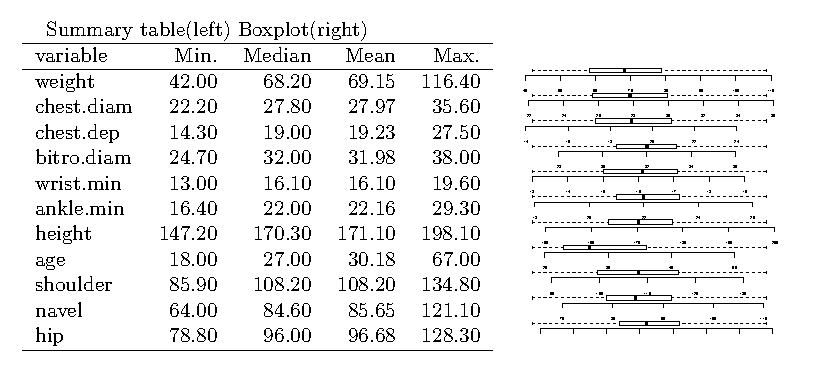
\includegraphics[width=0.9\textwidth]{summary_table}\\
These are the 11 out of 25 variables selected from the original dataset. Most of these 11 variables are symmetrically distributed except age. The mean of weight, height and age are 69.15kg, 171.10cm and 30.18 yr, respectively, which would suggest that the avarage subjects are middle and healthy.


%------------------------------------------------

\subsection{Outcome of Interest: Weight}

The initial reason the data was collected was to determine how well weight could be predicted between body build, weight, and girths. Using weight as the response variable, these data can be used to investigate the correspondence between frame size, girths, and weight of physically active young men and women that are within a normal weigth range. 
\begin{knitrout}
\definecolor{shadecolor}{rgb}{0.969, 0.969, 0.969}\color{fgcolor}
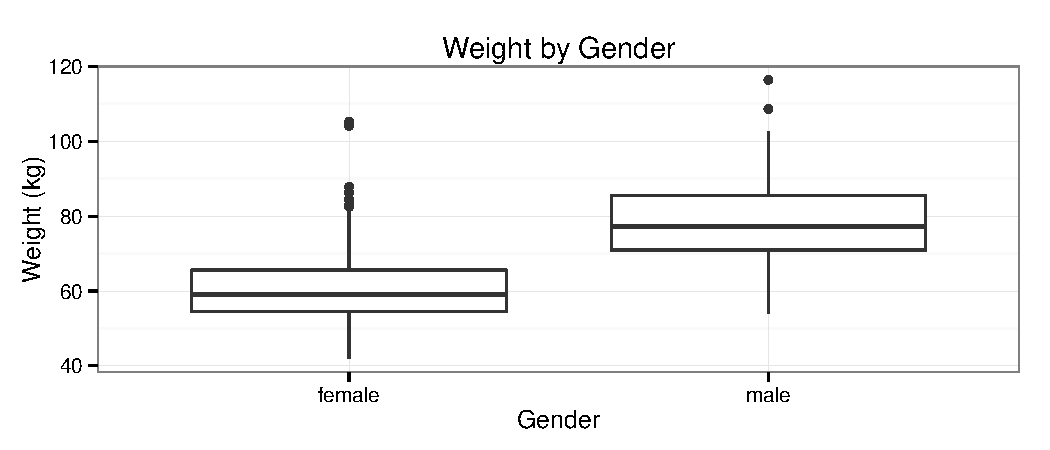
\includegraphics[width=\maxwidth]{figure/weight_plot} 

\end{knitrout}


%------------------------------------------------------------------

\subsection{Initial Multiple Linear Regression Model} % Emily

The initial model we are interested in fitting is of the form:\\

weight$_i = \beta_0 + \beta_1$ chest.diam$_{i} + \beta_2$ chest.dep$_{i} + \beta_3$ bitro.diam$_{i} + \beta_4$ wrist.min$_{i}$ + $\beta_5$ ankle.min$_{i} + \beta_6$ height$_{i}$ \\

The paper attached with the dataset mentioned multiple models one could use, we chose this as our base model, due to the fact that the model had variables across the entire body, included measurements of depth, girth and diameter and contained a reasonable amount of variables. The variables are: chest diameter (at mid-expiration level), chest depth (between spine and sternum at mid-expiration), bitrochanteric diameter (distance between both trochanters),  wrist minimum girth (average of right and left girths), ankle minimum girth (average), and height.

\begin{knitrout}
\definecolor{shadecolor}{rgb}{0.969, 0.969, 0.969}\color{fgcolor}\begin{kframe}
\begin{verbatim}
## (Intercept)  chest.diam   chest.dep  bitro.diam   wrist.min   ankle.min 
##    -109.890       1.340       1.537       1.196       1.113       1.152 
##      height 
##       0.177
\end{verbatim}
\end{kframe}
\end{knitrout}


Our model indicates that the expected weight when all variables are 0 is -110 (which does not make sense in this context). Furthermore the expected change in weight for a 1 unit change in chest.diam, holding all other variables constant, is 1.34 kgs. The expected change in weight for a 1 unit change in chest.dep, holding all other variables constant, is 1.54 kgs., etc. Note that chest depth has the largest impact on weight. In addition to the coefficients, the model has an R-squared value of 0.8882 which implies that our model explains 88.82\% of the variation in weight. This model seems like a good tool to predict weight given these measurements, but can we find a better one?

%------------------------------------------------
\newpage

\section{Individual Analyses}

%------------------------------------------------
\subsection{Model Diagnostics (Nick)} %Nick



%------------------------------------------------
\newpage

\subsection{Model Selection (Emily)} %Emily

\subsubsection{Initial Model}

As stated previously, the initial model we are interested in fitting is of the form:\\
weight$_i = \beta_0 + \beta_1$ chest.diam$_{i} + \beta_2$ chest.dep$_{i} + \beta_3$ bitro.diam$_{i} + \beta_4$ wrist.min$_{i} + \beta_5$ ankle.min$_{i} + \beta_6$ height$_{i}$




\begin{knitrout}
\definecolor{shadecolor}{rgb}{0.969, 0.969, 0.969}\color{fgcolor}\begin{kframe}
\begin{verbatim}
## (Intercept)  chest.diam   chest.dep  bitro.diam   wrist.min 
##    -109.890       1.340       1.537       1.196       1.113 
##   ankle.min      height 
##       1.152       0.177
\end{verbatim}
\end{kframe}
\end{knitrout}


This model indicates that the expected change in weight for a 1 unit change in chest.diam, holding all other variables constant, is 1.34 kgs. The expected change in weight for a 1 unit change in chest.dep, holding all other variables constant, is 1.54 kgs., etc. Note that chest depth has the largest impact on weight. In addition to the coefficients, the R-squared value of 0.8882 implies that our model explains 88.82\% of the variation in weight and the $P$-values for each variable and for the model are significant. This model seems like a good tool to predict weight given these measurements, but are there better ones?

\subsubsection{Model Selection}

We are building a model to predict weight given various body measurements. Before running random models, we need to determine what predictors to use. The predictors needed in our models are age, height and gender. These variables contribute significantly to weight. The predictors we will allow in model selection are the initial predictors: chest diameter, chest depth and bitro diameter. In addition to these variables, pelvic bredth, shoulder, chest, waist, hip and thigh will be used. I chose to allow these predictors in my model since these are directly associated with weight (e.g. waist). However, for the other models we will fit, we will let ``R" do it's work.

\subsubsection{Criterion}

The Information Criterions we will be using to evaluate our models are Akaike Information Crierion (AIC), Bayes Information Criterion (BIC), adjusted $R^2$ and Predictive Residual Sum of Squares (PReSS). In short, AIC and BIC measure goodness-of-fit through residual sum of squares (log likelihoods) and penalizes the model size; the smaller the AIC/BIC, the better. Adjusted $R^2$ adjusts $R^2$ so that the model is penalized for adding more predictors; the higher the value of the adjusted $R^2$ the better. Finally, PRESS is a summary measure focused on prediction; the lower the value of PRESS, the better.
\begin{eqnarray*}
\text{AIC} &=& n\log \left(\dfrac{RSS}{n}\right) + 2(p +1)\\
\text{BIC} &=& n\log \left(\dfrac{RSS}{n}\right) + (p + 1) \log(n)\\
\text{adj}R^2 &=& 1 - \dfrac{n - 1}{n - p - 1}(1 - R^2)\\
\end{eqnarray*}
\begin{eqnarray*}
\text{PRESS} &=& \sum{\left(\dfrac{\hat{\epsilon}_i}{1 - h_{ii}}\right)^2}
\end{eqnarray*}

\subsubsection{Methods in R}

There are multiple methods built into different packages in R for Model Selection. To illustrate these, we will use the variables:  height, wrist.min, ankle.min and chest.



\textbf{stepAIC()}\\

The R function found in the package ``MASS" called ``stepAIC()" performs stepwise model selection by AIC. This will output the initial model and the final model (model of best fit determined by this method), and the steps taken. In the output below we can see that this method suggests using a different model that doesn't contain wrist.diam.\\




\texttt{Initial Model: weight ~ height + wrist.diam + ankle.diam + chest\\
Final Model: weight ~ height + ankle.diam + chest\\
\begin{tabular}{r r r r r r r}
        &  Step & Df & Deviance & Resid. Df & Resid. Dev & AIC \\
1  &            &      &        &  502 &  13294.14 & 1666.150 \\
2 & - wrist.diam & 1 & 47.90427 & 503 &   13342.05 & 1665.974
\end{tabular}
}


\textbf{leaps()}\\

The R package ``leaps" contains a function ``regsubsets()". This method performs an exhaustive search of models and plots the $R^2$ criterion by variables and subset size. The class ``summary.regsubsets" outputs an object with multiple elements, including adjusted $R^2$ and BIC. Furthermore, the plots below plot the  
BIC and Adjusted $R^2$ values against each subset of variables. 

\begin{knitrout}
\definecolor{shadecolor}{rgb}{0.969, 0.969, 0.969}\color{fgcolor}
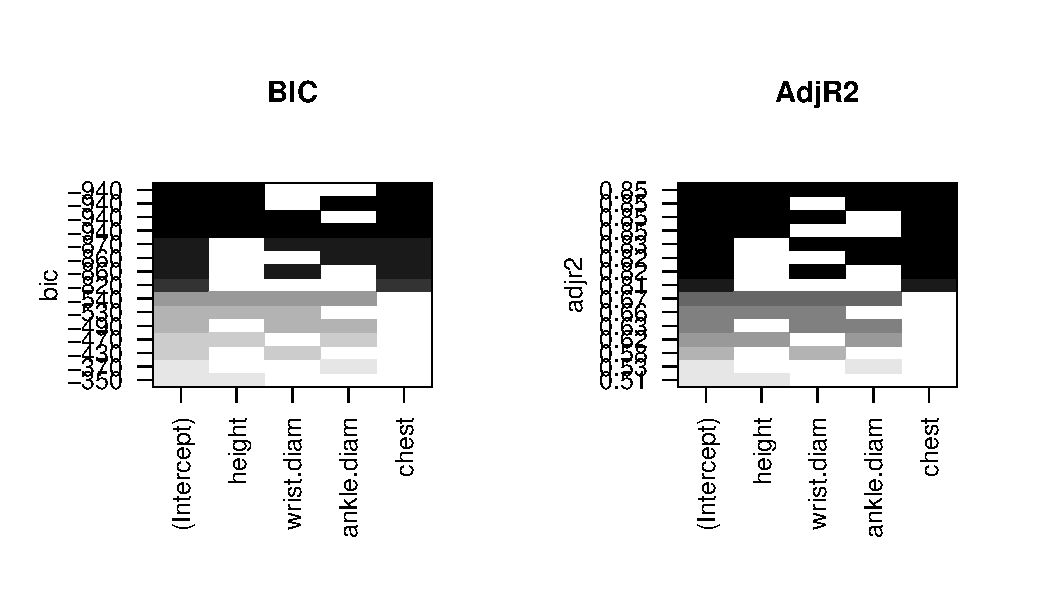
\includegraphics[width=\maxwidth]{figure/leap} 

\end{knitrout}


In these plots, for example, the BIC plot is implying the best model is using height and chest as predictors. On the other hand, the AdjR2 plot is saying all variables give the best fit. Using both of these plots together, one might conclude height, ankle.diam and chest would be the best fit. This conclsion agrees with our analysis using stepAIC.

\subsubsection{Model Selection in Action}




The Model Selection Lab will explain how to obtain the models summarized in Table 1.     

\textbf{Table 1}\\

\begin{center}
\begin{tabular}{|r|c|c|c|c|r|}
  \hline
MLR\# & AIC & BIC & PRESS & Adjusted $R^2$ & Method \\ 
  \hline
all & 2216 & 2326 & 2384 & 0.9753 & \text{all variables  from dataset used} \\ \hline
i & 2970 & 3004 & 10405 & 0.8869 & \text{suggested by paper} \\ \hline
1 & 2256 & 2319 & 2560 & 0.9727 & \text{suggested by paper}\\ \hline
2 & 2402 & 2441 & 3408 & 0.9632 & \text{my model}\\ \hline
3 & 2206 & 2282 & 2329 & 0.9754 & \text{stepAIC} \\ \hline
4 & 2195 & \textcolor{blue}{2271} & \textcolor{blue}{2281} & \textcolor{blue}{0.9759} & \text{stepAIC and adjustments} \\ \hline
5 & 2207 & 2292 & 2335 & 0.9755 &\text{leaps (adj} $R^2$) \\ \hline
6 & \textcolor{red}{2189} & 2278 & \textcolor{red}{2255} & \textcolor{red}{0.9764}  & \text{leaps(adj} $R^2$) \text{and adjustments}\\ \hline
7 & 2213 & 2272 & 2353 & 0.9749 & \text{leaps(BIC)} \\ \hline
8 & \textcolor{blue}{2205} & \textcolor{red}{2264} & 2316 & 0.9753 & \text{leaps(BIC) and adjustments}\\ \hline
\end{tabular}
\end{center}

Base on Table 1, we can see that each criteria yields different results. It is up to our discretion to choose a model. \textcolor{red}{Red} corresponds to the best value, of all 10 models, for that criteria, \textcolor{blue}{blue} is the second best. Since AIC and PRESS are lowest in MLR6, the adjusted $R^2$ is the largest, and the BIC is close to the best and second best values, I would choose MLR6 as the model of best fit. MLR6 is of the form:\\ 

weight$_i = \beta_0 + \beta_1$ pelvic.bredth$_{i} + \beta_2$ bitro.diam$_{i} + \beta_3$ chest.dep$_{i} + \beta_4$ chest$.diam_{i}$ + $\beta_5$ elbow.diam$_{i} + \beta_6$ knee.diam$_{i}$ + 
$\beta_7$ shoulder$_{i}$ + $\beta_7$ chest$_{i}$ + $\beta_8$ waist$_{i}$ + $\beta_9$ hip$_{i}$ + $\beta_{10}$ thigh$_{i}$ + $\beta_{11}$ bicep$_{i} + \beta_{12}$ forearm$_{i} + \beta_{13}$ knee$_{i} + \beta_{14}$ calf$_{i} +\beta_{15}$ age$_{i} + \beta_{16}$ height$_{i} + \beta_{17}$ gender$_{i} + \beta_{18}$ height$^2_{i}$. \\

Note in Table 1 the first and second lowest values for AIC, BIC and Press, and the first and second highest values for Adjusted $R^2$ were for stepAIC with adjustments and leaps with adjustments.

\subsubsection{Conclusion}
Model Selection truely is an art form. R can mechanically run through steps, interactions, combinations, etc. However, R cannot subjectively look at the variables to determine the absolute best model. To acheive the model of best fit, a combination of methods and human adjustment is necessary.

\newpage

%------------------------------------------------
\subsection{Logistic regression and Ada-Boosting (Yiding)}

\subsubsection{Logistic regression}

\textbf{AIC Method:} The procedure- Start from the full-fit model that include the all variables and then delete the one variable that would decrease the AIC most, and then delete another one.
\begin{table}[ht]
\centering
\resizebox{0.98\textwidth}{!}{
\begin{tabular}{rlc}
  \hline
  Step \# & Model & AIC \\ 
  \hline
  1 & $logi$(SEX)=WT+CDM+CDP+BDM+WR+ANK+HT+AGE+SHD+NAV+HIP & 110.35\\
  2 & $logi$(SEX)=WT+CDP+BDM+WR+ANK+HT+AGE+SHD+NAV+HIP & 108.36\\
  3 & $logi$(SEX)=WT+CDP+BDM+WR+HT+AGE+SHD+NAV+HIP & 106.45\\
  4 & $logi$(SEX)=CDP+BDM+WR+HT+AGE+SHD+NAV+HIP & 104.55\\
  5 & $logi$(SEX)=CDP+WR+HT+AGE+SHD+NAV+HIP & 102.69\\
  6 & $logi$(SEX)=CDP+WR+HT+AGE+SHD+HIP & 101.05\\
   \hline
\end{tabular}
}
\end{table}
\\
The final model: $logi(gender)=-62.14702 +0.29592\times chest.dep + 1.30672\times wrist.min + 0.20283\times height + 0.05411\times age + 0.44689\times shoulder - 0.50595\times hip$\\

\textbf{BIC Method:} The method start picking the variables that have highest posterior probabilities individually against null model and then add the secondary highest variables to the model.
\begin{table}[ht]
\centering
\resizebox{0.89\textwidth}{!}{
\begin{tabular}{rlrc}
  \hline
  Model \# & Model & BIC & Posterior prob\\ 
  \hline
  1 & $logi$(SEX)=WR+HT+SHD+HIP & -3033 & 0.453\\
  2 & $logi$(SEX)=WR+HT+AGE+SHD+HIP & -3031 & 0.157\\
  3 & $logi$(SEX)=CDP+WR+HT+AGE+SHD+HIP & -3031 & 0.151\\
  4 & $logi$(SEX)=WR+HT+SHD+NAV+HIP & -3031 & 0.142\\
  5 & $logi$(SEX)=WR+HT+SHD+HIP & -3029 & 0.047\\
   \hline
\end{tabular}
}
\end{table}

The model with least BIC and most posterior probability is model 1 and it includes $wrist, height, shoulder, hip$. The model is : $logi(gender)=-61.89401 + 1.42080\times wrist+ 0.19783\times height+0.46062\times shoulder-0.46046\times hip$\\

\textbf{Brief Summary:} When the model is small, according to the p-value of each variable, the BIC method peform better. Besides, the final model calculated by AIC includes some implausible variable, such that "age"--meaningless in reality and "chest.dep"--not significant. However, p-value is just one criterion to estimate the goodness of a model. What else perspectives should we consider?\\

\textbf{Check Goodness of Model}\\
\textsc{Linearity:} Checking the residuals can be useful for identifying potential outliers (observations not well fit by the model) as well as misspecified models. The larger the deviance, the poorer the fit.



\begin{knitrout}
\definecolor{shadecolor}{rgb}{0.969, 0.969, 0.969}\color{fgcolor}
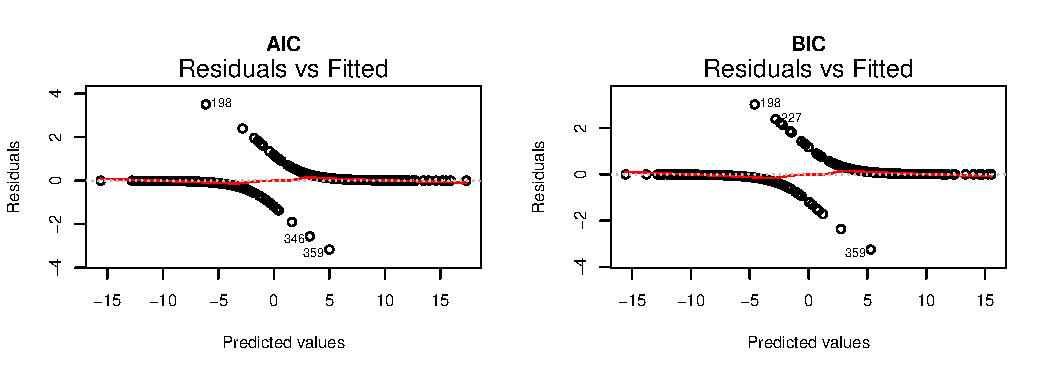
\includegraphics[width=\maxwidth]{figure/model_check} 

\end{knitrout}

Both model have a fairly good fit except several subjects that have high predicted probability in the center of x-axis.\\

\textsc{Quantifying Predictive Ability:} Usually, using 0.5 as a cutoff point to determine the prediced outcome is 1 or 0 by estimated probabilities is a quantified way of assessing the predictive ability. Similar to the cutoff method, the Receiver Operating Characteristic (ROC) curv is a very usful method to assess the predictive ability. It is a curve such that plotted based on the sensitivity against 1-specificity of a series cutoff points. The area under the ROC curve can give us insight into the predictive ability of the model. If $c(area)$ =  0.5 means model predicting at random and if $c$ = 1 indicates a very good predictive ability.\\
When Somers' $D_{xy}$ rank correlation = 0, $D_{xy}=2(c-0.5)= 0$, the model is making random prediction; when = 1, the model discriminates outcome perfectly.\\

\begin{knitrout}
\definecolor{shadecolor}{rgb}{0.969, 0.969, 0.969}\color{fgcolor}
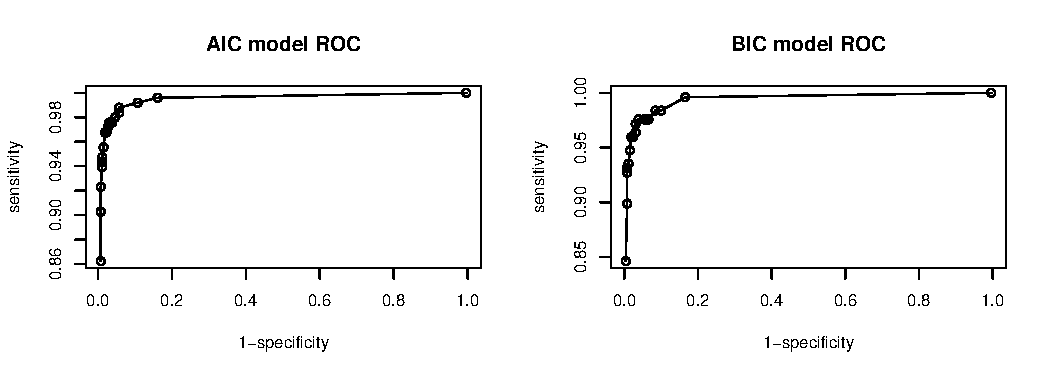
\includegraphics[width=\maxwidth]{figure/ROV_curve} 

\end{knitrout}


\begin{table}[ht]
\centering
\resizebox{0.45\textwidth}{!}{
\begin{tabular}{ccc}
  \hline
  Model  & Area ROC curve & Somers' $D_{xy}$\\ 
  \hline
  AIC & 0.9944721 & 0.9889443\\
  BIC & 0.9941607 & 0.9883214\\
   \hline
\end{tabular}
}
\end{table}

Both of them have a very good predictive ability, but from the perspective of efficiency, the BIC model is preferable. Because BIC model use fewer variables to achive the as high as AIC model's predictive ability. 
In reality, how the performance is depends on how the cutoff point been selected. The higher cutoff point you selected, the higher accuracy the prediction would be. However, the higher sensitivity would lead to a poor specificity.

\subsubsection{Ada-Boosting}

Ada-boosting is a tree based method to find a good classification stratagy to classify the data. Its key idea is to give more weight to the subjects that wrongly classified during last round of classification. This method is so powerful that one do not need to select cutoff point and model selection.\\
The algorithem of AdaBoost: \textit{Yoav.F, Robert E.S,A Short Introduction to Boosting, 1999.}\\
Given: $(x_1,y_1),...,(x_m,y_m)$ where $x_i \in X, y_i \in Y=\{-1,+1\}$\\
Initialize $D_1(i)=1/m$.\\
For $t=1,...,T$:\\
$\bullet$ Train weak learner using distribution $D_t$.\\
$\bullet$ Get weak hypothesis $h_t : X \rightarrow \{-1,+1\}$ with error $\epsilon_t=Pr_{i\sim D_t}\left[ h_t(x_i)\ne y_i \right]$\\
$\bullet$ Choose $\alpha_t=\frac{1}{2}ln\left(\frac{1-\epsilon_t}{\epsilon_t}\right)$\\
\[
D_{t+1}(i)=\frac{D_t(i)}{Z_t}\times
\left\{\begin{matrix}
e^{-\alpha_t} & \mbox{if $h_t(x_i)=y_i$}\\
e^{\alpha_t} & \mbox{if $h_t(x_i)\ne y_i$}
\end{matrix}
\right.
\]
where $Z_t$ is a normalization factor.\\
Output the final hypothesis:\\
$$H(x)=sign\left(\sum_{t=1}^{T}\alpha_t h_t(x)\right)$$
Conduct 5 rounds ada-boosting trainning on original data, AIC selected data and BIC selected data, using 1/2 of the data as trainning data and the rest 1/2 of data as test data.
\begin{table}[ht]
\centering
\resizebox{\textwidth}{!}{
\begin{tabular}{ccccc}
  \hline
  Round $\#$  & Original data & AIC data & BIC data\\
       & Sensitiviy; Specificity; Accuracy & Sensitiviy; Specificity; Accuracy & Sensitiviy; Specificity; Accuracy\\ \hline
    1 & 0.975; 0.925; 0.949 & 0.967; 0.962; 0.965 & 0.967; 0.947; 0.957\\
    2 & 0.953; 0.936; 0.945 & 0.953; 0.920; 0.937 & 0.961; 0.936; 0.949\\
    3 & 0.949; 0.951; 0.949 & 0.954; 0.959; 0.957 & 0.954; 0.959; 0.957\\
    4 & 0.983; 0.932; 0.957 & 0.983; 0.955; 0.961 & 0.983; 0.962; 0.972\\
    5 & 0.983; 0.924; 0.953 & 0.983; 0.931; 0.957 & 0.983; 0.947; 0.965\\
    Avarage & 0.969; 0.934; 0.951 & 0.968; 0.945; 0.955 & 0.970; 0.950; 0.960\\
  \hline

\end{tabular}
}
\end{table}
Ada-boosting is so powerful that without subsetting the data it can make a very good prediction with high sensitivity, specificity and accuracy, subsetting data according to the AIC and BIC model can improve the ada-boosting performance. The BIC data has a littel better performance than AIC model, since the data contains less variables, resulting a more efficient prediction.

\subsubsection{Conclusion}

As we see, ada-boosting cannot be a better and convinient way to make prediction. However, ada-boosting cannot make any inferences about each variables, which would result in some drawbacks such as blindly collect data and unefficiency caused by too many noise variables. In other words, if one needs to determine and make a strong inference about certain variables, like a car insurance company wants to determine whether a driver is a safe-driver or not base on his/her age, income etc., the logistic regression model is neccessary. Thus he/she should choose the tools according to his or her purposes.

%------------------------------------------------
\newpage

\subsection{Regression Trees: Differences in Males and Females (Liza)} %Liza

As we have shown in previous sections, males and females differ significantly in terms of weight and body measurements. However, the regression presented for predicting weight did not include a term for gender, citing that doing so would not add significantly to the model. My hypothesis is that separate models for males and females would be more appropriate based on the systematic differences in body shape and size between the genders. Using recursive partitioning, or regression tree analysis, I plan to explore what the most important variables are in predicting weight for the two genders both together and separately to see if there are differences in the way the data is divided based on the different body measurements sampled.


\begin{center}
\begin{figure}
\begin{knitrout}
\definecolor{shadecolor}{rgb}{0.969, 0.969, 0.969}\color{fgcolor}
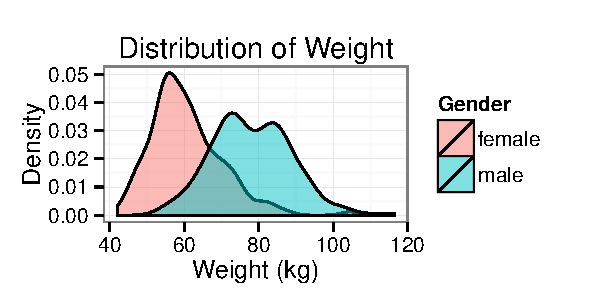
\includegraphics[width=\maxwidth]{figure/wdt} 

\end{knitrout}

\vspace{-10pt}
\caption{Figure 1: Desnsity distribution of Weight for males and females}
\end{figure}
\end{center}

\subsubsection{Tree 1: Males and Females} 
To explore whether gender is an important dividing variable for the entire dataset, I first grew a regression tree with all of the data. As shown in the regression tree below, a split was not produced based on gender of the subjects. Variables used in this tree are waist girth, chest girth, hip girth, knee girth and knee diameter.

\begin{knitrout}
\definecolor{shadecolor}{rgb}{0.969, 0.969, 0.969}\color{fgcolor}
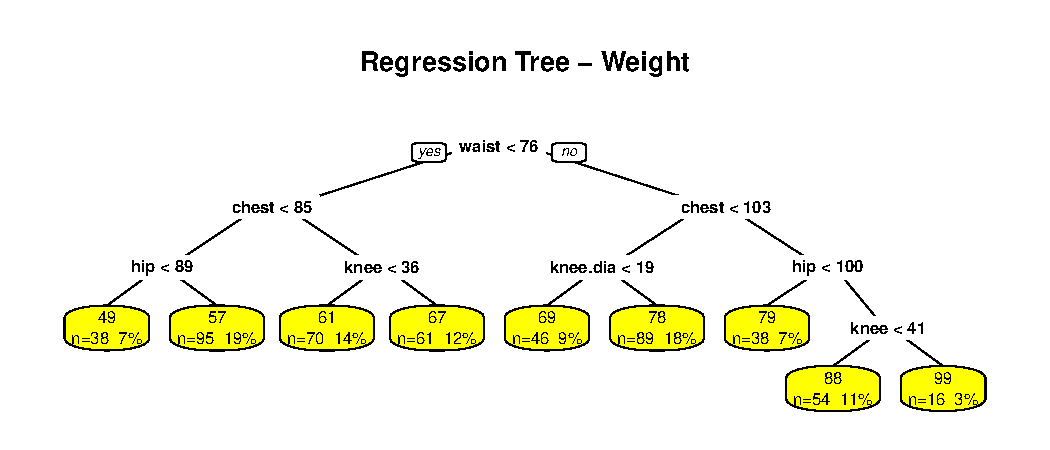
\includegraphics[width=\maxwidth]{figure/wt} 

\end{knitrout}


\subsubsection{Tree 2: Males} 
Even though the full dataset did not utilize gender to partition the data, it might be informative to see if we obtain different trees by subsetting the data by gender. Next, I produced a regression tree with weight as the dependent variable for males only using all available body measurement variables. The CP tables showed us that at 5 splits we obtain a minimum relative error, therefore we were able to prune the tree to a reasonable size to avoid overfitting the data (Figure 2a). The final variables used to produce the pruned tree were hip girth and shoulder girth.

\begin{knitrout}
\definecolor{shadecolor}{rgb}{0.969, 0.969, 0.969}\color{fgcolor}\begin{kframe}
\begin{verbatim}
## 
## Regression tree:
## rpart(formula = weight ~ ., data = bodym, method = "anova")
## 
## Variables actually used in tree construction:
## [1] hip      shoulder
## 
## Root node error: 27188/247 = 110
## 
## n= 247 
## 
##      CP nsplit rel error xerror  xstd
## 1 0.552      0      1.00   1.00 0.094
## 2 0.129      1      0.45   0.47 0.049
## 3 0.069      2      0.32   0.36 0.041
## 4 0.032      3      0.25   0.31 0.030
## 5 0.025      4      0.22   0.32 0.029
## 6 0.014      5      0.19   0.31 0.028
\end{verbatim}
\end{kframe}
\end{knitrout}

\begin{figure}
\begin{knitrout}
\definecolor{shadecolor}{rgb}{0.969, 0.969, 0.969}\color{fgcolor}
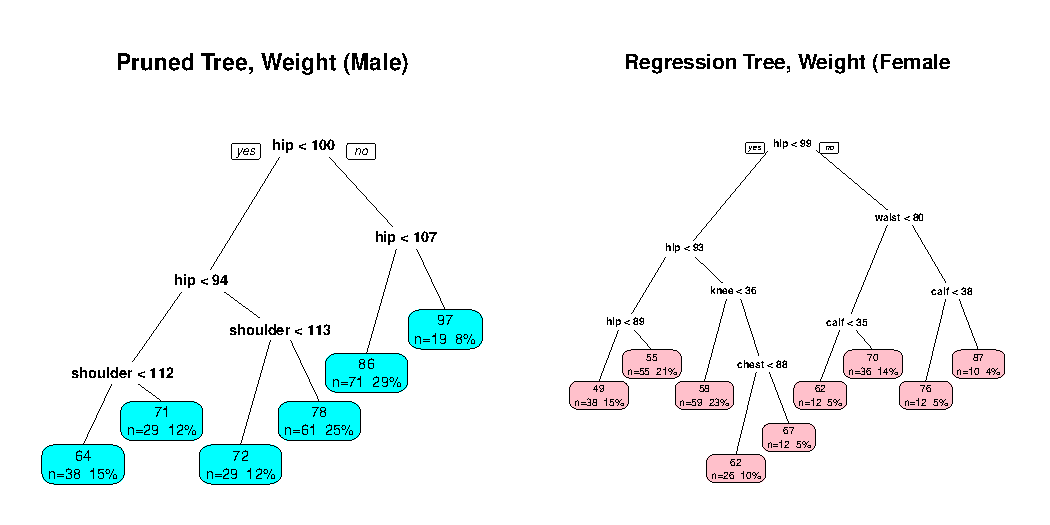
\includegraphics[width=\maxwidth]{figure/mtrees} 

\end{knitrout}

\caption{Figure 2: a. Pruned regression tree for male weight. b. Regression tree for female weight.}
\end{figure}
\subsubsection{Tree 3: Females} 
The regression tree for the female subset (Figure 2b) does not reach a minimum relative error before the final node and therefore did not need pruning. The variables used to produce this tree vary significantly in number and type from the male tree. They are: hip girth, knee girth, calf girth, chest girth, and waist girth. In fact, the only variable the female tree and the pruned male tree have in common is shoulder girth.

\begin{knitrout}
\definecolor{shadecolor}{rgb}{0.969, 0.969, 0.969}\color{fgcolor}\begin{kframe}
\begin{verbatim}
## 
## Regression tree:
## rpart(formula = weight ~ ., data = bodyf, method = "anova")
## 
## Variables actually used in tree construction:
## [1] calf  chest hip   knee  waist
## 
## Root node error: 23948/260 = 92
## 
## n= 260 
## 
##      CP nsplit rel error xerror  xstd
## 1 0.516      0      1.00   1.01 0.134
## 2 0.129      1      0.48   0.54 0.072
## 3 0.112      2      0.35   0.41 0.069
## 4 0.031      3      0.24   0.30 0.040
## 5 0.028      4      0.21   0.29 0.039
## 6 0.027      5      0.18   0.28 0.039
## 7 0.019      6      0.16   0.26 0.039
## 8 0.010      7      0.14   0.25 0.038
## 9 0.010      8      0.13   0.23 0.038
\end{verbatim}
\end{kframe}
\end{knitrout}


\subsubsection{Conclusion}
While regression trees are not intended to produce a model for prediction, they can be quite useful in elucidating the most important variables for partitioning data. Here we found that these variables differed significantly between men and women, perhaps suggesting that separate models for predicting weight would be more appropriate and potentially more accurate than one general model for both genders. Further analysis would be needed to test this hypothesis, specifically model fitting and selction for subsets of the data by gender. One could then show whether these separate models have better predictive power than one combined model.

%------------------------------------------------------------------------

\newpage

\section{Conclusion/ Discussion}


\end{document}
